%\RequirePackage{currfile}
\documentclass[12pt]{beamer}
\usepackage[utf8]{inputenc}
\usepackage[spanish]{babel}
\usepackage{standalone}
\usepackage{color}
\usepackage{siunitx}
\usepackage{hyperref}
\usepackage[outdir=./]{epstopdf}
%\hypersetup{colorlinks,linkcolor=,urlcolor=blue}
%\hypersetup{colorlinks,urlcolor=blue}
\usepackage{anyfontsize}
\usepackage{lmodern}
\usepackage{xcolor,soul}
\usepackage{etoolbox}
\usepackage{amsmath}
\usepackage{amsthm}
\usepackage{mathtools}
\usepackage{tcolorbox}
\usepackage{physics}
\usepackage{multicol}
\usepackage{bookmark}
\usepackage{longtable}
\usepackage{listings}
\usepackage{cancel}
\usepackage{wrapfig}
\usepackage{empheq}
\usepackage{graphicx}
\usepackage{tikz}
\usetikzlibrary{calc, patterns, matrix, backgrounds, decorations,shapes, arrows.meta}
\usepackage[autostyle,spanish=mexican]{csquotes}
\usepackage[os=win]{menukeys}
\usepackage{pifont}
\usepackage{pbox}
\usepackage{bm}
\usepackage{caption}
\captionsetup{font=scriptsize,labelfont=scriptsize}
%\usepackage[sfdefault]{roboto}  %% Option 'sfdefault' only if the base font of the document is to be sans serif

%Sección de definición de colores
\definecolor{ao}{rgb}{0.0, 0.5, 0.0}
\definecolor{bisque}{rgb}{1.0, 0.89, 0.77}
\definecolor{amber}{rgb}{1.0, 0.75, 0.0}
\definecolor{armygreen}{rgb}{0.29, 0.33, 0.13}
\definecolor{alizarin}{rgb}{0.82, 0.1, 0.26}
\definecolor{cadetblue}{rgb}{0.37, 0.62, 0.63}
\definecolor{deepblue}{rgb}{0,0,0.5}
\definecolor{brown}{rgb}{0.59, 0.29, 0.0}
\definecolor{OliveGreen}{rgb}{0,0.25,0}
\definecolor{mycolor}{rgb}{0.122, 0.435, 0.698}

\newcommand*{\boxcolor}{orange}
\makeatletter
\newcommand{\boxedcolor}[1]{\textcolor{\boxcolor}{%
\tikz[baseline={([yshift=-1ex]current bounding box.center)}] \node [rectangle, minimum width=1ex, thick, rounded corners,draw] {\normalcolor\m@th$\displaystyle#1$};}}
 \makeatother

 \newcommand*\widefbox[1]{\fbox{\hspace{2em}#1\hspace{2em}}}

\newtcbox{\mybox}{on line,
  colframe=mycolor,colback=mycolor!10!white,
  boxrule=0.5pt,arc=4pt,boxsep=0pt,left=6pt,right=6pt,top=6pt,bottom=6pt}

\usefonttheme[onlymath]{serif}
%Sección de definición de nuevos comandos

\newcommand*{\TitleParbox}[1]{\parbox[c]{1.75cm}{\raggedright #1}}%
\newcommand{\python}{\texttt{python}}
\newcommand{\textoazul}[1]{\textcolor{blue}{#1}}
\newcommand{\azulfuerte}[1]{\textcolor{blue}{\textbf{#1}}}
\newcommand{\funcionazul}[1]{\textcolor{blue}{\textbf{\texttt{#1}}}}
\newcommand{\ptilde}[1]{\ensuremath{{#1}^{\prime}}}
\newcommand{\stilde}[1]{\ensuremath{{#1}^{\prime \prime}}}
\newcommand{\ttilde}[1]{\ensuremath{{#1}^{\prime \prime \prime}}}
\newcommand{\ntilde}[2]{\ensuremath{{#1}^{(#2)}}}
\renewcommand{\arraystretch}{1.5}

\newcounter{saveenumi}
\newcommand{\seti}{\setcounter{saveenumi}{\value{enumi}}}
\newcommand{\conti}{\setcounter{enumi}{\value{saveenumi}}}
\renewcommand{\rmdefault}{cmr}% cmr = Computer Modern Roman

\linespread{1.5}

\usefonttheme{professionalfonts}
%\usefonttheme{serif}
\DeclareGraphicsExtensions{.pdf,.png,.jpg}

%Sección para el tema de beamer, con el theme, usercolortheme y sección de footers
\mode<presentation>
{
  \usetheme{Berlin}
  
  %\useoutertheme{infolines}
  \useoutertheme{default}
  \usecolortheme{beaver}
  \setbeamercovered{invisible}
  % or whatever (possibly just delete it)
  \setbeamertemplate{section in toc}[sections numbered]
  \setbeamertemplate{subsection in toc}[subsections numbered]
  \setbeamertemplate{subsection in toc}{\leavevmode\leftskip=3.2em\rlap{\hskip-2em\inserttocsectionnumber.\inserttocsubsectionnumber}\inserttocsubsection\par}
  \setbeamercolor{section in toc}{fg=blue}
  \setbeamercolor{subsection in toc}{fg=blue}
  \setbeamercolor{frametitle}{fg=blue}
  \setbeamertemplate{caption}[numbered]

  \setbeamertemplate{footline}
  \beamertemplatenavigationsymbolsempty
  \setbeamertemplate{headline}{}
}

\makeatletter
\setbeamercolor{section in foot}{bg=gray!30, fg=black!90!orange}
\setbeamercolor{subsection in foot}{bg=blue!30!yellow, fg=red}
\setbeamertemplate{footline}
{
  \leavevmode%
  \hbox{%
  \begin{beamercolorbox}[wd=.333333\paperwidth,ht=2.25ex,dp=1ex,center]{section in foot}%
    \usebeamerfont{section in foot} \insertsection
  \end{beamercolorbox}}%
  \begin{beamercolorbox}[wd=.333333\paperwidth,ht=2.25ex,dp=1ex,center]{subsection in foot}%
    \usebeamerfont{subsection in foot}  \insertsubsection
  \end{beamercolorbox}%
  \begin{beamercolorbox}[wd=.333333\paperwidth,ht=2.25ex,dp=1ex,right]{date in head/foot}%
    \usebeamerfont{date in head/foot} \insertshortdate{} \hspace*{2em}
    \insertframenumber{} / \inserttotalframenumber \hspace*{2ex} 
  \end{beamercolorbox}}%
  \vskip0pt%
\makeatother  

\makeatletter
\patchcmd{\beamer@sectionintoc}
  {\vfill}
  {\vskip\itemsep}
  {}
  {}
\makeatother


\title{\large{Aplicaciones de la Transformada de Laplace}}
\subtitle{Tema 6 - Transformadas Integrales}
\author{M. en C. Gustavo Contreras Mayén}
\date{}
\institute{Facultad de Ciencias - UNAM}
\titlegraphic{
\includegraphics[width=1.75cm]{../Imagenes/escudo-facultad-ciencias}\hspace*{4.75cm}~%
   
\includegraphics[width=1.75cm]{../Imagenes/escudo-unam}
}
\setbeamertemplate{navigation symbols}{}
\lstset{language=Mathematica}
\lstset{basicstyle={\sffamily\footnotesize},
  numbers=left,
  numberstyle=\tiny\color{gray},
  numbersep=5pt,
  breaklines=true,
  captionpos={t},
  frame={lines},
  rulecolor=\color{black},
  framerule=0.5pt,
  columns=flexible,
  tabsize=2,
  escapeinside=||
}
\lstnewenvironment{mat}
{\lstset{language=mathematica,mathescape,columns=flexible}}
{}
\usepackage{scalerel}
\def\scaleint#1{\vcenter{\hbox{\scaleto[3ex]{\displaystyle\int}{#1}}}}
\def\bs{\mkern-12mu}

\begin{document}
\maketitle
\fontsize{14}{14}\selectfont
\spanishdecimal{.}

\section*{Contenido}
\frame[allowframebreaks]{\tableofcontents[currentsection, hideallsubsections]}
%Ref. Penney. Cp. 7 Ecs. Diferenciales

\section{La Transformada de Laplace}
\frame{\tableofcontents[currentsection, hideothersubsections]}
\subsection{Definiciones}

\begin{frame}
\frametitle{La Transformada de Laplace}
Dada una función $f(t)$ definida para toda $t \geq 0$, \emph{la transformada de Laplace} de $f$ es la función $F$ definida por:
\pause
\begin{align*}
F(s) = \mathcal{L} \left\{ f(t) \right\} = \scaleint{5ex}_{\bs 0}^{\infty} \exp(-s \, t) \, f(t) \dd{t}
\end{align*}
para todo valor de $s$ en los cuales la integral impropia converge.
\end{frame}
\begin{frame}
\frametitle{Transformada inversa de Laplace}
Si $F(s)$ es la transformada de Laplace de alguna función continua $f(t)$, \pause entonces $f(t)$ está determinada de manera única.
\\
\bigskip
\pause
Si $F(s) = \mathcal{L} \left\{ f(t) \right\}$, entonces se llama $f(t)$ \emph{la transformada inversa de Laplace}:
\begin{align*}
f(t) = \mathcal{L}^{-1} \left\{ F(s) \right\}
\end{align*}
\end{frame}
\begin{frame}
\frametitle{Transformada de derivadas de orden superior}
Si las funciones $f$, $\ptilde{f}$, $\stilde{f}, \ldots, \ntilde{f}{n}$ son continuas y suaves en tramos para $t \geq 0$, y que cada una es de orden exponencial, con los mismos valores de $M$ y $c$.
\\
\bigskip
\pause
Entonces, la transformada de la derivada de orden $n$ de $f$ existe cuando $s > c$ y:
\end{frame}
\begin{frame}
\frametitle{Transformada de derivadas de orden superior}
Se tiene que:
\begin{align*}
\mathcal{L} \left\{ \ntilde{f}{n} (t) \right\} &= s^{n} \, F(s) - s^{s-1} f(0) - s^{n-2} \, \ptilde{f}(0) + \ldots \\[1em]
&- \ldots \ntilde{f}{n-2}(0) - \ntilde{f}{n-1}(0)
\end{align*}

\end{frame}

\section{Resonancia y factores cuadráticos repetidos}
\frame{\tableofcontents[currentsection, hideothersubsections]}
\subsection{Transformadas de interés}

\begin{frame}
\frametitle{Transformadas inversas de utilidad}
Las siguientes dos transformadas inversas de Laplace son útiles para invertir fracciones parciales al caso de factores cuadráticos repetidos:
\begin{align}
L^{-1} \left\{ \dfrac{1}{(s^{2} + k^{2})} \right\} &= \dfrac{1}{ k} \, \sin k \, t \label{eq:ecuacion_07_03_16} \\[0.5em]
L^{-1} \left\{ \dfrac{1}{(s^{2} + k^{2})^{2}} \right\} &= \dfrac{1}{2 \, k^{3}} \, (\sin k \, t - k \, t \, \cos k \, t) \label{eq:ecuacion_07_03_17}
\end{align}
\end{frame}
\begin{frame}
\frametitle{Fenómeno de resonancia}
Debido a la presencia de los términos $t \, \sin k \, t$ y $t \, \cos k \, t$ en las ecs. (\ref{eq:ecuacion_07_03_16}) y (\ref{eq:ecuacion_07_03_17}), un factor cuadrático repetido comúnmente indica la presencia del fenómeno de resonancia en un sistema mecánico no amortiguado o en un sistema eléctrico.
\end{frame}

\subsection{Primer ejemplo}

\begin{frame}
\frametitle{Enunciado}
Resuelve el siguiente problema con valores iniciales:
\begin{align*}
\stilde{x} + \omega_{0}^{2} \, x = F_{0} \, \sin \omega \, t, \hspace{1cm} x(0) = \ptilde{x} (0) = 0
\end{align*}
que determinan las oscilaciones forzadas no amortiguadas de una masa sujeta a un resorte.
\end{frame}
\begin{frame}
\frametitle{Aplicando la transformada de Laplace}
Aplicando la transformada de Laplace a la ED, se obtiene la ecuación:
\pause
\begin{align*}
s^{2} \, X(s) + \omega^{2} \, X(s) = \dfrac{F_{0} \, \omega}{s^{2} + \omega^{2}}
\end{align*}
\pause
Recordemos la notación $X(s)$, representa la transformada de Laplace de la función $x(t)$.
\end{frame}
\begin{frame}
\frametitle{Organizando la expresión}
Por lo que al despejar $X(s)$, tenemos que:
\pause
\begin{align*}
X(s) = \dfrac{F_{0} \, \omega}{(s^{2} + \omega^{2})(s^{2} + \omega_{0}^{2})}
\end{align*}
\pause
Por lo que habrá que revisar los dos casos:
\setbeamercolor{item projected}{bg=blue!70!black,fg=yellow}
\setbeamertemplate{enumerate items}[circle]
\begin{enumerate}[<+->]
\item $\omega \neq \omega_{0}$.
\item $\omega = \omega_{0}$.
\end{enumerate}
\end{frame}
\begin{frame}
\frametitle{Caso especial $\omega \neq \omega_{0}$}
Si $\omega \neq \omega_{0}$, se encuentra que:
\begin{align*}
X(s) = \dfrac{F_{0} \, \omega}{\omega^{2} - \omega_{0}^{2}} \, \left( \dfrac{1}{s^{2}+ \omega_{0}^{2}} - \dfrac{1}{s^{2} + \omega^{2}} \right)
\end{align*}
\end{frame}
\begin{frame}
\frametitle{Obteniendo la solución}
De esta manera al aplicar la transformada inversa de Laplace, ec. (\ref{eq:ecuacion_07_03_16}), se concluye que la solución es:
\pause
\begin{align*}
x(t) = \dfrac{F_{0} \, \omega}{\omega^{2} - \omega_{0}^{2}} \left( \dfrac{1}{\omega_{0}} \sin \omega_{0} \, t - \dfrac{1}{\omega} \, \sin \omega \, t \right)
\end{align*}
\end{frame}
\begin{frame}
\frametitle{Caso $\omega = \omega_{0}$}
Pero si $\omega = \omega_{0}$, se tiene que:
\pause
\begin{align*}
X(s) = \dfrac{F_{0} \, \omega_{0}}{(s^{2} + \omega^{2})^{2}}
\end{align*}
\end{frame}
\begin{frame}
\frametitle{Solución}
Aplicando la transformada inversa de Laplace, la ec. (\ref{eq:ecuacion_07_03_17}) obtenemos la solución de resonancia:
\pause
\begin{align}
x(t) = \dfrac{F_{0}}{2 \, \omega_{0}^{2}} \, (\sin \omega_{0} \, t - \omega_{0} \, t \, \cos \omega_{0} \, t )
\label{eq:ecuacion_07_03_18}
\end{align}
\pause
En la figura (\ref{fig_figura_07_03_04}), con $F_{0}=1$ y $\omega=0.5$ se puede ver la solución de resonancia y las curvas envolventes.
\end{frame}
\begin{frame}
\frametitle{Gráfica de la solución}
\begin{figure}[H]
    \centering
    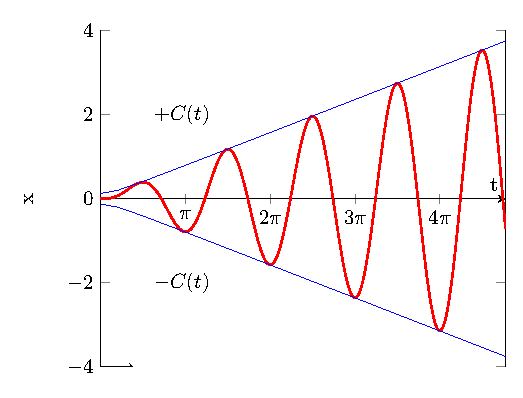
\includegraphics[scale=0.95]{Imagenes/sist_masa_resorte_resonancia_plot_01.eps}
    \caption{La solución de resonancia junto con sus curvas envolventes.}
    \label{fig_figura_07_03_04}
\end{figure}
\end{frame}
\begin{frame}
\frametitle{Curvas envolventes}
La curva solución definida por la ec. (\ref{eq:ecuacion_07_03_18}) oscila una y otra vez, como vemos en la figura (\ref{fig_figura_07_03_04}) entre dos \enquote{rectas envolventes}: $x = \pm \, C(t)$, que se obtienen al escribir la ec. (\ref{eq:ecuacion_07_03_18}) en la forma
\begin{align*}
x(t) =  A(t) \, \cos \omega_{0} \, t +  B(t) \, \sin \omega_{0 \, t}
\end{align*}
\end{frame}
\begin{frame}
\frametitle{Amplitud de la solución}
Definiendo entonces la usual \enquote{amplitud}
\begin{align*}
C = \sqrt{A^{2} +  B^{2}}
\end{align*}
\pause
En este caso se encuentra que
\begin{align*}
C(t) = \dfrac{F_{0}}{2 \, \omega_{0}^{2}} \, \sqrt{\omega_{0}^{2} \, t^{2} + 1}
\end{align*}
\end{frame}

\subsection{Segundo ejemplo}

\begin{frame}
\frametitle{Enunciado Segundo Ejemplo}
Con un sistema masa resorte amortiguador, considera los valores de $m = 1$, $k = 9.04$, $c= 0.4$ y $F(t) =  6 \, \exp(-t/5) \, \cos 3 \, t$.
\\
\bigskip
Con las condiciones iniciales:
\begin{align*}
x(0) = \ptilde{x}(0) = 0
\end{align*}
\end{frame}
\begin{frame}
\frametitle{Preguntas por resolver}
\setbeamercolor{item projected}{bg=blue!70!black,fg=yellow}
\setbeamertemplate{enumerate items}[circle]
\begin{enumerate}[<+->]
\item Resuelve el problema para obtener el desplazamiento $x(t)$.
\item ¿Cuál es el valor máximo de la amplitud?
\item Grafica el desplazamiento $x(t)$ y discute tus resultados.
\end{enumerate}
\end{frame}
\begin{frame}
\frametitle{La EDO de inicio}
Partimos de la siguiente EDO:
\begin{align*}
m \, \stilde{x} + c \, \ptilde{x} + k \, x = F(t)
\end{align*}
\pause
Con los valores señalados en el enunciado, tenemos la EDO
\begin{align*}
\stilde{x} + 0.4 \, \ptilde{x} + 9.04 \, x = 6 \, \exp\left( -\dfrac{t}{5}\right) \, \cos 3 \, t
\end{align*}
Con las condiciones iniciales:
\begin{align*}
x(0) = \ptilde{x}(0) = 0
\end{align*}
\end{frame}
\begin{frame}
\frametitle{Aplicando la TL}
Aplicamos la transformada de Laplace en ambos lados de la EDO:
\begin{align*}
L \big[\stilde{x}\big] &+ L\big[0.4 \, \ptilde{x}\big] + L \big[9.04 \, x\big] = \\[0.5em]
=& L \left[ 6 \, \exp \left( -\dfrac{t}{5}\right) \, \cos 3 \, t \right]
\end{align*}
\pause
Que al aplicar las propiedades de la TL revisadas en el material de trabajo, obtenemos lo siguiente:
\end{frame}
\begin{frame}
\frametitle{Usando las propiedades}
\begin{eqnarray*}
L \big[\stilde{x}\big] &=& s^{2} \, X(s) - s \, f(0) - \ptilde{f}(0) \\[0.5em] \pause
L \big[0.4 \, \ptilde{x}\big] &=& 0. 4 \big( s \, X(s) - f(0)\big) \\[0.5em] \pause
L \big[9.04 \, x\big] &=& 9.04 \, X(s)
\end{eqnarray*}
\end{frame}
\begin{frame}
\frametitle{Usando las propiedades}
\begin{eqnarray*}
L \left[ 6 \, \exp \left( -\dfrac{t}{5}\right) \, \cos 3 \, t \right] &=& 6 \, L \left[\exp \left( -\dfrac{t}{5}\right) \, \cos 3 \, t \right] \\[0.5em] \pause
&=& 6 \left( \dfrac{s - (-1/5)}{\big[s - 1/5\big]^{2} + 3^{2}} \right) \\[0.5em] \pause
&=& \dfrac{6 \, (s + 1/5)}{9 + (s + 1/5)^{2}}
\end{eqnarray*}
\end{frame}
\begin{frame}
\frametitle{Ocupando las condiciones iniciales}
\begin{align*}
x(0) = \ptilde{x}(0) = 0
\end{align*}
\pause
La ecuación es:
\begin{align*}
s^{2} \, X(s) + 0.4 \, s \, X(s) + 9.04 \, X(s) = \dfrac{6 \, (s + 1/5)}{9 + (s + 1/5)^{2}}
\end{align*}
\pause
Que al ordenar los términos para despejar $X(s)$, obtenemos:
\end{frame}
\begin{frame}
\frametitle{Ecuación algebraica en $X(s)$}
La ecuación es:
\begin{align*}
X(s) = \dfrac{6 \, (s + 1/5)}{\big[s^{2} + 0.4 \, s + 9.04\big] \big[9 + (s + 1/5)^{2}\big]}
\end{align*}
\end{frame}
\begin{frame}
\frametitle{Aplicando al transformada inversa}
Ahora debemos de aplicar la transformada inversa de Laplace para obtener la solución $x(t)$:
\\
\bigskip
\pause
De nuevo ocupamos las propiedades de la transformada inversa de Laplace:
\end{frame}
\begin{frame}
\frametitle{Resultado obtenido}
El resultado que se obtiene es:
\pause
\begin{align*}
x(t) = t \, \exp (-t/5)
\end{align*}
Con lo que hemos resuelto el primer inciso del problema.
\end{frame}
\begin{frame}
\frametitle{Obteniendo el valor máximo}
Para obtener el valor máximo de la función $x(t)$, aplicamos lo que ya sabemos de Cálculo I: \pause obtenemos la derivada de primer orden con respecto a $t$, para encontrar las raíces (en qué punto(s) se anula).
\begin{align*}
\ptilde{x}(t) = 0
\end{align*}
\end{frame}
\begin{frame}
\frametitle{Derivando la función}
La derivada es:
\begin{align*}
\ptilde{x}(t) = \exp(-t/5) - \dfrac{t}{5} \, \exp(-t/5) 
\end{align*}
\pause
Que al hacer:
\begin{align*}
\exp(-t/5) - \dfrac{t}{5} \, \exp(-t/5) = 0
\end{align*}
\end{frame}
\begin{frame}
\frametitle{Obteniendo la(s) raíz(ces)}
Así:
\begin{eqnarray*}
5 \, \exp(-t/5) - t \, \exp(-t/5) &=& 0  \\[0.5em] \pause
\exp(-t/5) (5 - t) &=& 0 \\[0.5em] \pause
(5 - t) &=& 0 \\[0.5em] \pause
t &=& 5
\end{eqnarray*}
\end{frame}
\begin{frame}
\frametitle{Signo de la segunda derivada}
Al derivar nuevamente $x(t)$ y evaluar la segunda derivada con la raíz encontrada, veremos cómo es el signo:
\begin{align*}
\stilde{x}(t) = -\dfrac{2}{5} \, \exp(-t/5) + \dfrac{1}{25} \, \exp(-t/5) \, t
\end{align*}
\pause
Que al evaluar en la raíz $t = 5$, nos devuelve: \pause
\begin{align*}
\stilde{x}(t=5) = - \dfrac{1}{5 \, e} < 0
\end{align*}
\pause
Por lo que tenemos el máximo de la función en $t = 5$.
\end{frame}
\begin{frame}
\frametitle{El valor máximo de la función}
Ahora evaluamos la raíz en $x(t)$, y obtenemos:
\begin{align*}
x(t=5) &= 5 \, \exp (-5/5) = \\[0.5em]
&= \dfrac{5}{e}
\end{align*}
Que representa el valor máximo de la amplitud de la función $x(t)$. \pause Ya hemos resuelto el segundo inciso.
\end{frame}
\begin{frame}
\frametitle{Gráfica de la función $x(t)$}
Ocupamos cualquier programa para graficar la función $x(t)$, puede ser directamente con \LaTeX, \emph{Mathematica}, \emph{MatLab}, o incluso usando programación con  \python.
\end{frame}
\begin{frame}
\frametitle{Obteniendo la gráfica}
\begin{figure}
    \centering
    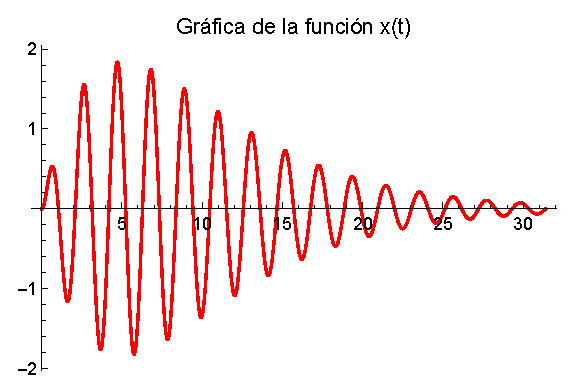
\includegraphics[scale=1]{Imagenes/Ejemplo_Resonancia_01.eps}
    \caption{Solución de $x(t)$ vs $t$}
\end{figure}
\end{frame}
\begin{frame}
\frametitle{Intepretando la gráfica}
Vemos que hay un intervalo en donde se presenta un incremento de la amplitud, se alcanza el máximo de la misma en $t = 5$, para luego ir disminuyendo conforme avanza el tiempo.
\\
\bigskip
\pause
Podemos hacer un estudio adicional para encontrar más información.
\end{frame}
\begin{frame}
\frametitle{Obteniendo una envolvente}
Es posible determinar una curva que \enquote{rodea} a la solución $x(t)$ \pause, para determinar la curva, podemos ocupar los valores en cada cresta de $x(t)$, de tal forma que si tomamos el valor absoluto, tendremos el doble de puntos y con ello, mejorar la aproximación de la curva.
\end{frame}
\begin{frame}
\frametitle{Graficando $\abs{x(t)}$}
\begin{figure}
    \centering
    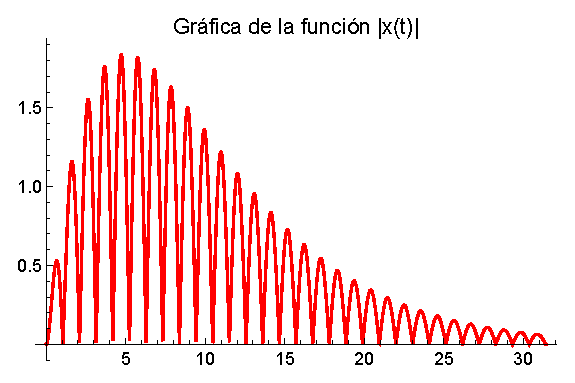
\includegraphics[scale=1]{Imagenes/Ejemplo_Resonancia_02.eps}
    \caption{Al tomar el valor absoluto, se tendrán más puntos para la aproximación.}
\end{figure}
\end{frame}
\begin{frame}
\frametitle{Obteniendo la envolvente}
\begin{figure}
    \centering
    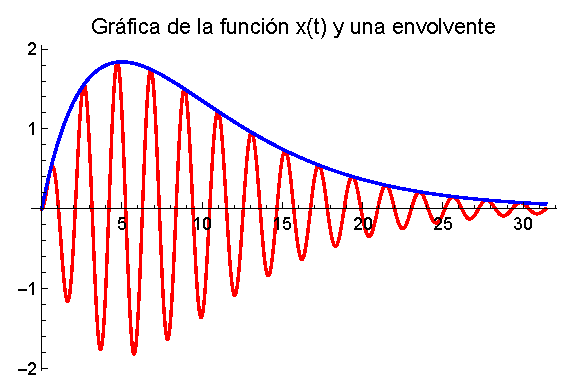
\includegraphics[scale=1]{Imagenes/Ejemplo_Resonancia_03.eps}
    \caption{La curva en azul es la envolvente de $x(t)$.}
\end{figure}
\end{frame}
\begin{frame}
\frametitle{Ventaja de la simetría}
Al ser $x(t)$ simétrica con respecto a $y = 0$, la curva envolvente para valores negativos, tendrá un signo negativo con respecto a los valores positivos.
\end{frame}
\begin{frame}
\frametitle{Dos curvas envolventes}
\begin{figure}
    \centering
    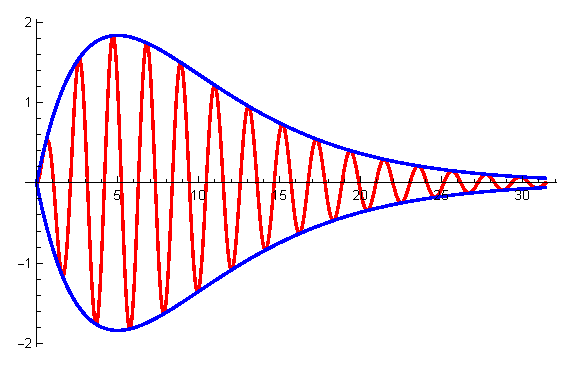
\includegraphics[scale=1]{Imagenes/Ejemplo_Resonancia_04.eps}
    \caption{Las curvas envolventes de $x(t)$.}
\end{figure}
\end{frame}
\begin{frame}
\frametitle{El resultado extendido}
\begin{figure}
    \centering
    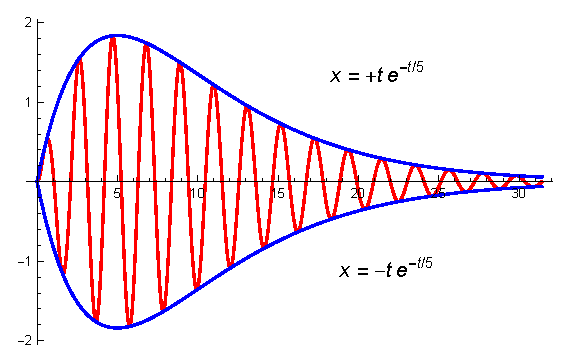
\includegraphics[scale=1]{Imagenes/Ejemplo_Resonancia_05.eps}
    \caption{Las curvas envolventes de $x(t)$ como función de $t$.}
\end{figure}
\end{frame}

\section{Masas acopladas}
\frame{\tableofcontents[currentsection, hideothersubsections]}
\subsection{Ejemplo 1}

\begin{frame}
\frametitle{Enunciado del ejercicio}
Dos masas, $m_{1}$ y $m_{2}$, están unidas a dos resortes, $A$ y $B$, de masa insignificante cuyas constantes de resorte son $k_{1}$ y $k_{2}$, respectivamente, los resortes se fijan como se ve en la figura (\ref{fig:figura_dos_masas_01}).
\end{frame}
\begin{frame}
\frametitle{Sistema de dos masas}
\begin{figure}
    \centering
    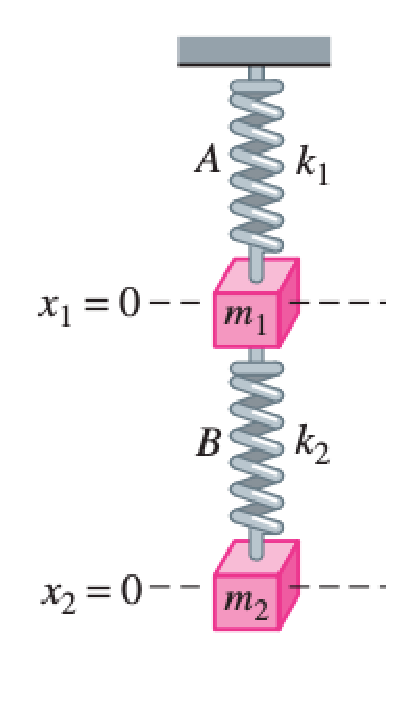
\includegraphics[scale=0.35]{Imagenes/Ejercicio_Dos_Masas_01.eps}
    \caption{El sistema de dos masas acopladas mediante resortes.}
    \label{fig:figura_dos_masas_01}
\end{figure}
\end{frame}
\begin{frame}
\frametitle{Enunciado del ejercicio}
Sean $x_{1}(t)$ y $x_{2}(t)$ los desplazamientos verticales de las masas respecto a sus posiciones de equilibrio.
\\
\bigskip
\pause
Cuando el sistema está en movimiento, el resorte $B$ está sujeto a elongación y compresión;
por lo que su elongación neta es $x_{2} - x_{1}$.
\end{frame}
\begin{frame}
\frametitle{Enunciado del ejercicio}
Por tanto, se deduce de la ley de Hooke que los resortes $A$ y $B$ ejercen fuerzas $-k_{1} \, x_{1}$ y $k_{2} (x_{2} - x_{1})$, respectivamente, en $m_{1}$.
\\
\bigskip
\pause
Si ninguna fuerza externa se aplica al sistema y si ninguna fuerza de amortiguamiento está
presente, entonces la fuerza neta en $m_{1}$ es
\begin{align*}
-k_{1} \, x_{1} + k_{2} (x_{2} - x_{1})
\end{align*}
\end{frame}
\begin{frame}
\frametitle{Sistema de dos masas}
\begin{figure}
    \centering
    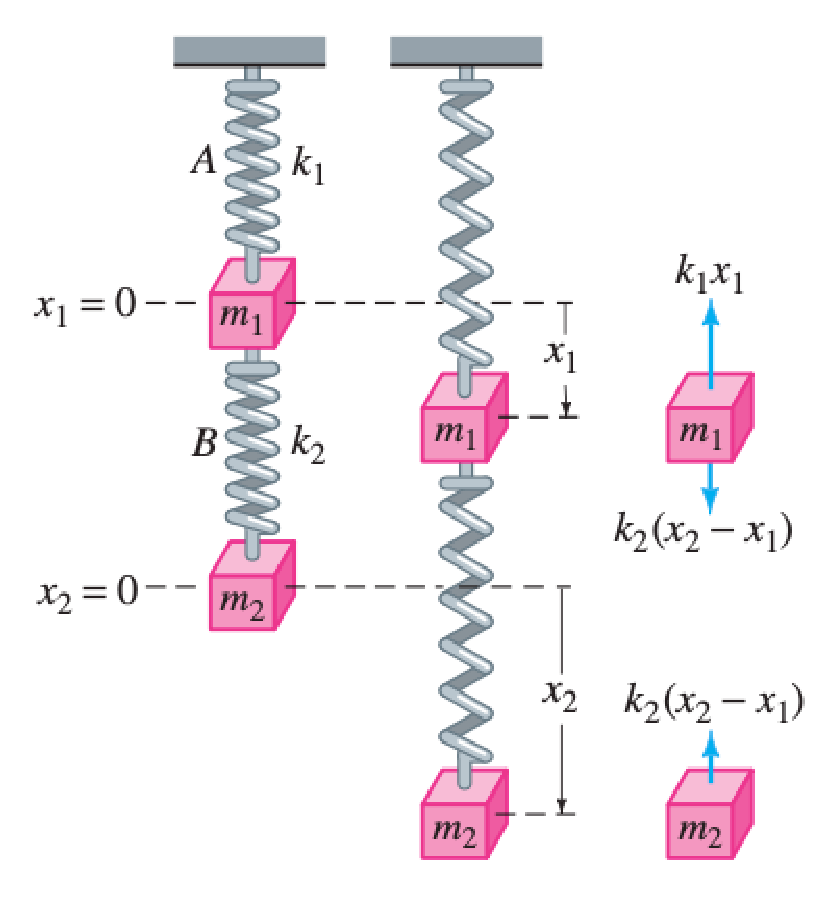
\includegraphics[scale=0.35]{Imagenes/Ejercicio_Dos_Masas_02.eps}
    \caption{El sistema en reposo, en movimiento y las fuerzas.}
    \label{fig:figura_dos_masas_02}
\end{figure}
\end{frame}
\begin{frame}
\frametitle{Ecuación de movimiento}
Por la segunda ley de Newton podemos escribir:
\begin{align*}
m_{1} \, \dv[2]{x_{1}}{t} = - k_{1} \, x_{1} + k_{2} (x_{2} - x_{1})
\end{align*}
\pause
De manera análoga, la fuerza neta ejercida en la masa $m_{2}$ se debe solo a la elongación neta de $B$.
\end{frame}
\begin{frame}
\frametitle{Ecuación de movimiento}
Es decir, $-k_{2} (x_{2} - x_{1})$. Por lo que:
\begin{align*}
m_{2} \, \dv[2]{x_{2}}{t} = - k_{2} \, (x_{2} - x_{1})
\end{align*}
\pause
Tenemos entonces un sistema acoplado:
\end{frame}
\begin{frame}
\frametitle{Sistema acoplado de masas}
El sistema de EDO que determina el movimiento de las masas es:
\begin{align*}
m_{1} \, \stilde{x}_{1} &= - k_{1} \, x_{1} + k_{2} (x_{2} - x_{1}) \\[0.5em]
m_{2} \, \stilde{x}_{2} &= - k_{2} \, (x_{2} - x_{1})
\end{align*}
\end{frame}
\begin{frame}
\frametitle{Condiciones del problema}
\textbf{Resuelve el sistema anterior}, considerando que: $k_{1} = 6$, $k_{2} = 4$, $m_{1} = m_{2} = 1$ y que las masas comienzan a moverse desde sus posiciones de equilibrio con velocidades unitarias opuestas.
\end{frame}
\begin{frame}
\frametitle{El problema a resolver}
Se tiene el siguiente sistema:
\begin{table}
\begin{tabular}{l l l l l }
$\stilde{x}_{1}$ & $+ 10 \, x_{1}$ &  & $- 4 \, x_{2}$ & $= 0$ \\[0.5em]
 & $-4 \, x_{1}$ & $+\stilde{x}_{2}$ & $+ 4 \, x_{2}$ & $=0$
\end{tabular}
\end{table}
sujeta a 
\begin{align*}
x_{1}(0) = 0, \hspace{0.3cm} \ptilde{x}_{1}(0) = 1, \hspace{0.3cm} x_{2}(0) = 0, \hspace{0.3cm} \ptilde{x}_{2}(0) = -1
\end{align*}
\end{frame}
\begin{frame}
\frametitle{Aplicamos la transformada de Laplace}
Se aplica la transformada de Laplace en cada ecuación para obtener: \pause
\begin{align*}
s^{2} \, X_{1}(s) {-} s \, x_{1}(0) {-} \ptilde{x}_{1}(0) {+} 10 \, X_{1}(s) {-} 4 \, X_{2}(s) = 0 \\[0.5em]
- 4 \, X_{1}(s) {+} s^{2} \, X_{2}(s) {-} s \, x_{2}(0) {-} \ptilde{x}_{2}(0) {+} 4 \, X_{2}(s) = 0
\end{align*}
donde $X_{1}(s) = L \big[x_{1} (t)\big]$ y $X_{2}(s) = L \big[x_{2} (t)\big]$, respectivamente.
\end{frame}
\begin{frame}
\frametitle{El sistema acoplado}
El sistema anterior es equivalente a:
\begin{table}
\begin{tabular}{r r l }
$(s^{2} + 10) \, X_{1}(s)-$ & $4 \, X_{2}(s)$ & $=1$ \\[0.5em]
$-4 \, X_{1}(s)+$ &$(s^{2} + 4) \, X_{2}(s)$ & $=-1$
\end{tabular}
\end{table}
\end{frame}
\begin{frame}
\frametitle{Resolviendo para $X_{1}(s)$}
Usando fracciones parciales:
\begin{align*}
X_{1}(s) = \dfrac{s^{2}}{(s^{2} + 2)(s^{2} + 12)} = - \dfrac{1/5}{s^{2} + 2} + \dfrac{6/5}{s^{2} + 12}
\end{align*}
\pause
Por lo que podemos ahora aplicar la transformada inversa de Laplace para obtener el desplazamiento de $x_{1}$:
\end{frame}
\begin{frame}
\frametitle{Aplicando la transformada inversa}
\begin{eqnarray*}
x_{1}(t) &=& \! -\dfrac{1}{5 \sqrt{2}} L^{-1} \left[ \dfrac{\sqrt{2}}{s^{2} + 2} \right] {+} \dfrac{6}{5 \sqrt{12}} \, L^{-1} \left[ \dfrac{\sqrt{12}}{s^{2} + 12} \right] \\[0.5em] \pause
&=& - \dfrac{\sqrt{2}}{10} \, \sin \sqrt{2} \, t + \dfrac{\sqrt{3}}{5} \, \sin 2 \, \sqrt{3} \, t
\end{eqnarray*}
\end{frame}
\begin{frame}
\frametitle{Resolviendo para $X_{2}(s)$}
Al sustituir la expresión para $X_{1}(s)$ en la primera ecuación del sistema, se obtiene:
\begin{align*}
X_{2}(s) = - \dfrac{s^{2} + 6}{(s^{2} + 2)(s^{2} + 12)} = - \dfrac{2/5}{s^{2} + 2} - \dfrac{3/5}{s^{2} + 12}
\end{align*}
\pause
De igual manera, aplicamos la transformada inversa de Laplace para obtener $x_{2}(t)$.
\end{frame}
\begin{frame}
\frametitle{Aplicando la transformada inversa}
\begin{eqnarray*}
x_{2}(t) &=& \! -\dfrac{2}{5 \sqrt{2}} L^{-1} \left[ \dfrac{\sqrt{2}}{s^{2} + 2} \right] {-} \dfrac{3}{5 \sqrt{12}} L^{-1} \left[ \dfrac{\sqrt{12}}{s^{2} + 12} \right] \\[0.5em] \pause
&=& - \dfrac{\sqrt{2}}{5} \, \sin \sqrt{2} \, t - \dfrac{\sqrt{3}}{10} \, \sin 2 \, \sqrt{3} \, t
\end{eqnarray*}
\end{frame}
\begin{frame}
\frametitle{Solución al sistema acoplado}
La solución al sistema acoplado es:
\begin{align*}
x_{1}(t) &= - \dfrac{\sqrt{2}}{10} \, \sin \sqrt{2} \, t + \dfrac{\sqrt{3}}{5} \, \sin 2 \, \sqrt{3} \, t \\[0.5em]
x_{2}(t) &= - \dfrac{\sqrt{2}}{5} \, \sin \sqrt{2} \, t - \dfrac{\sqrt{3}}{10} \, \sin 2 \, \sqrt{3} \, t
\end{align*}
\end{frame}
\begin{frame}
\frametitle{Gráfica de los resultados}
Conociendo las soluciones $x_{1}(t)$ y $x_{2}(t)$, ahora podemos presentar una gráfica de las funciones, como se puede ver en la siguiente figura (\ref{fig:plot_dos_masas_01}):
\end{frame}
\begin{frame}
\frametitle{Gráficas de las funciones}
\begin{figure}
    \centering
    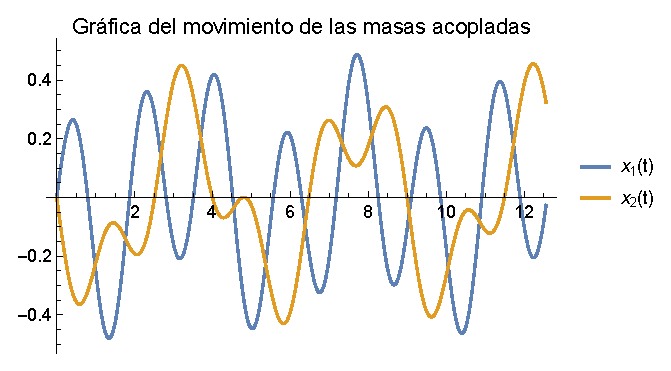
\includegraphics[scale=1]{Imagenes/Ejercicio_masas_acopladas_01.eps}
    \caption{Movimiento de las masas $m_{1}$ y $m_{2}$.}
    \label{fig:plot_dos_masas_01}
\end{figure}
\end{frame}

% \section{Usando \texttt{Mathematica}}
% \frame{\tableofcontents[currentsection, hideothersubsections]}
% \subsection{Primer ejercicio resonancia}

% \begin{frame}
% \frametitle{Usando paquetería para resolver}
% A continuación resolveremos los mismos ejercicios ocupando \texttt{Mathematica}, en donde se verá la relativa facilidad para implementar el código y obtener la solución de cada uno de los ejercicios.
% \end{frame}
% \begin{frame}
% \frametitle{Nota importante}
% Es importante señalar que se debe de tener conocimiento en la sintaxis para utilizar \texttt{Mathematica}, no es la intención de revisar cada sentencia que se mostrará, pero consultando la documentación podrán interpretar qué es lo que está haciendo cada línea.
% \end{frame}
% \begin{frame}
% \frametitle{Primer ejemplo resonancia}
% El primer ejemplo que resolvimos es el siguiente:
% \begin{align*}
% \stilde{x} + \omega_{0}^{2} \, x = F_{0} \, \sin \omega \, t, \hspace{1cm} x(0) = \ptilde{x} (0) = 0
% \end{align*}
% \end{frame}
% \begin{frame}
% \frametitle{Estrategia de solución}
% Es importante que siempre tengamos planteada una estructura de la solución antes de escribir una instrucción en \texttt{Mathematica} como en otros programas o lenguajes.
% \end{frame}
% \begin{frame}
% \frametitle{Pasos de solución}
% Ocuparemos los siguientes pasos:
% \setbeamercolor{item projected}{bg=blue!70!black,fg=yellow}
% \setbeamertemplate{enumerate items}[circle]
% \begin{enumerate}[<+->]
% \item \textbf{Paso 1: } La función \funcionazul{LaplaceTransform} requiere como argumento: la función a transformar, y los argumentos $t$, $s$.
% \item \textbf{Paso 2: } Aplicamos las condiciones iniciales del problema.
% \item \textbf{Paso 3: } Se resuelve la ecuación algebraica para $X(s)$, usando la función \funcionazul{Solve}.
% \seti
% \end{enumerate}
% \end{frame}
% \begin{frame}
% \frametitle{Pasos de solución}
% Una vez conocida $X(s)$, aplicamos la transformada inversa de Laplace
% \setbeamercolor{item projected}{bg=blue!70!black,fg=yellow}
% \setbeamertemplate{enumerate items}[circle]
% \begin{enumerate}[<+->]
% \conti
% \item La variable \texttt{\textbf{sol}} tendrá el resultado que devuelve la función \funcionazul{InverseLaplaceTransform}, que ocupa como primer argumento la solución algebraica del \textbf{Paso 3}, punto importante: el valor se anota a mano; los otros argumentos son $s$, $t$.
% \seti
% \end{enumerate}
% \end{frame}
% \begin{frame}
% \frametitle{Pasos de solución}
% \setbeamercolor{item projected}{bg=blue!70!black,fg=yellow}
% \setbeamertemplate{enumerate items}[circle]
% \begin{enumerate}[<+->]
% \setcounter{enumi}{4}
% \item En este mismo paso, se ocupa la función \funcionazul{Simplify} que usa como argumento, el inciso anterior, esta función reducirá lo más posible el resultado.
% \item La función \funcionazul{Expand}, extiende el resultado en términos de las potencias involucradas.
% \end{enumerate}
% \end{frame}
% \begin{frame}
% \frametitle{Pasos de solución}
% \setbeamercolor{item projected}{bg=blue!70!black,fg=yellow}
% \setbeamertemplate{enumerate items}[circle]
% \begin{enumerate}[<+->]
% \setcounter{enumi}{6}
% \item Se grafica la solución mediante la función \funcionazul{Plot}, que ocupa de argumentos: la función a graficar, la variable independiente, así como el intervalo de graficación. 
% \end{enumerate}
% \end{frame}
% \begin{frame}[fragile]
% \frametitle{El código en \texttt{Mathematica}}
% Con $F_{0} = 1$ y $\omega = 1.25$
% \\
% \bigskip
% \begin{lstlisting}[language=Mathematica]
% paso1 = LaplaceTransform[x''[t]+(1.25)^2 x[t] == Sin[1.25t],t,s] |\pause|
% paso2 = paso1 /. {x[0] -> 0, x'[0] -> 0} |\pause|
% paso3 = Solve[paso2, LaplaceTransform[x[t], t, s]]
% \end{lstlisting}
% \pause
% El \textbf{Paso 3} nos devuelve: $X(s) = 1.25/(1.5625 + s^{2})$, que se debe de ocupar para el uso de la transformada inversa de Laplace.
% \end{frame}
% \begin{frame}[fragile]
% \frametitle{El código en \texttt{Mathematica}}
% \begin{lstlisting}[language=Mathematica]
% sol = Simplify[InverseLaplaceTransform[1.25/(1.5625 + s^2)^2, s, t]] // Expand |\pause|
% Plot[sol, {t, 0, 10 Pi}, PlotLabel -> "Grafica de la solucion x(t)", LabelStyle -> Directive[FontSize -> 12], PlotStyle -> {Red}]
% \end{lstlisting}
% \end{frame}
% \begin{frame}
% \frametitle{Grafica obtenida}
% \begin{figure}[H]
%     \centering
%     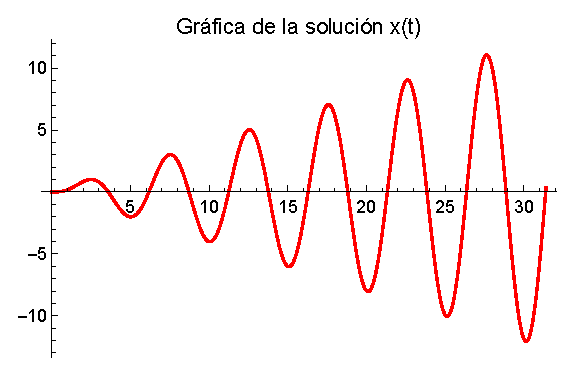
\includegraphics[scale=1]{Imagenes/Ejemplo_Resonancia_01_01.eps}
%     \caption{Solución obtenida con \texttt{Mathematica}.}
% \end{figure}
% \end{frame}
% \begin{frame}
% \frametitle{Rectas envolventes}
% De la solución \enquote{a mano} sabemos que hay un par de rectas envolventes, conocemos la expresión de éstas, por lo que ahora podemos incluirlas en el código y así visualizarlas.
% \end{frame}
% \begin{frame}[fragile]
% \frametitle{El código en \texttt{Mathematica}}
% \begin{lstlisting}[language=Mathematica]
% recta1 = Sqrt[(1.25)^2 t ^2 + 1]/(2*(1.25)^2) |\pause|
% Plot[{sol, recta1, -recta1 }, {t, 0, 10 Pi}, PlotStyle -> {{Red, Dashing[None]}, {Blue, Dashing[None]}, {Blue, Dashing[None]}}]
% \end{lstlisting}
% \end{frame}
% \begin{frame}
% \frametitle{Grafica obtenida}
% \begin{figure}[H]
%     \centering
%     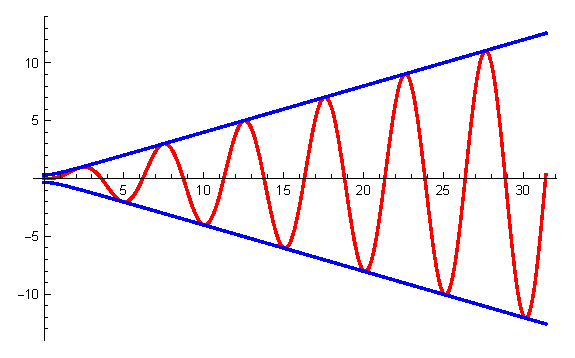
\includegraphics[scale=1]{Imagenes/Ejemplo_Resonancia_01_02.eps}
%     \caption{Solución obtenida con \texttt{Mathematica} y las envolventes.}
% \end{figure}
% \end{frame}
% \begin{frame}
% \frametitle{Agregando texto a la gráfica}
% Con \texttt{Mathematica} es posible agregar texto (entre otros elementos) y darle un mejor formato a la gráfica, no requiere el uso de comandos.
% \\
% \bigskip
% \pause
% Aunque también se pueden agregar elementos desde el código, pero como primer paso, el uso de las herramientas de dibujo facilita el trabajo.
% \end{frame}
% \begin{frame}
% \frametitle{Grafica obtenida con texto}
% \begin{figure}[H]
%     \centering
%     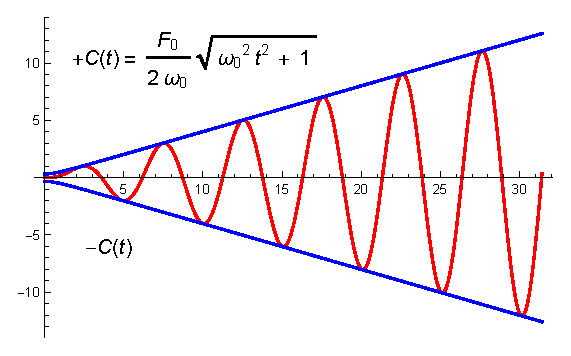
\includegraphics[scale=1]{Imagenes/Ejemplo_Resonancia_01_03.eps}
%     \caption{Solución obtenida con \texttt{Mathematica}, las envolventes y texto agregado.}
% \end{figure}
% \end{frame}
% \subsection{Segundo ejercicio de resonancia}
% \begin{frame}
% \frametitle{Segundo ejemplo de resonancia}
% Ahora resolveremos el segundo ejercicio de resonancia:
% \begin{align*}
% \stilde{x} + 0.4 \, \ptilde{x} + 9.04 \, x = 6 \, \exp\left( -\dfrac{t}{5}\right) \, \cos 3 \, t
% \end{align*}
% Con las condiciones iniciales:
% \begin{align*}
% x(0) = \ptilde{x}(0) = 0
% \end{align*}    
% \end{frame}
% \begin{frame}[fragile]
% \frametitle{Código en \texttt{Mathematica}}
% \begin{lstlisting}[language=Mathematica]
% EDO01 = x''[t]+0.4x'[t]+9.04x[t]== 6 Exp[-t/5]Cos[3 t] |\pause|
% paso1 = LaplaceTransform[EDO01,t,s] |\pause|
% paso2 = paso1/.{x[0]->0,x'[0]->0} |\pause|
% paso3 = Solve[paso2,LaplaceTransform[x[t],t,s]]
% \end{lstlisting}
% \end{frame}
% \begin{frame}
% \frametitle{Solución para $X(s)$}
% El \textbf{Paso 3} devuelve el valor:
% \begin{align*}
% X(s) = \dfrac{6 \, (s + 0.2)}{\left(s^2 + 0.4 \, s + 9.04\right) \left((s + 0.2)^2 + 9\right)}
% \end{align*}
% que se debe de ocupar para la transformada inversa de Laplace.
% \end{frame}
% \begin{frame}[fragile]
% \frametitle{Código en \texttt{Mathematica}}
% \begin{lstlisting}[language=Mathematica]
% sol = Simplify[InverseLaplaceTransform[(6 (0.2 +s))/((9.04 +0.4s+s^2)(9+(0.2+s)^2)),s,t]]//Expand |\pause|
% Plot[sol,{t,0,10 Pi},PlotLabel->"Grafica de la funcion x(t)", LabelStyle->Directive[FontSize->12],PlotStyle->{Red}]
% \end{lstlisting}
% \end{frame}
% \begin{frame}
% \frametitle{Gráfica de la solución $x(t)$}
% \begin{figure}[H]
%     \centering
%     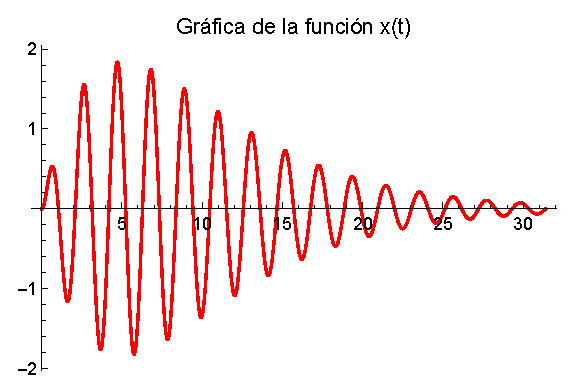
\includegraphics[scale=1]{Imagenes/Ejemplo_Resonancia_01.eps}
%     \caption{Solución obtenida con \texttt{Mathematica}.}
% \end{figure}
% \end{frame}
% \begin{frame}[fragile]
% \frametitle{Para encontrar el valor máximo}
% Para determinar el máximo de la función $x(t)$, ocupando \texttt{Mathematica} siguiendo el análisis que en la solución \enquote{a mano}: \pause
% \begin{lstlisting}[language=Mathematica]
% curva = t* Exp[-t/5] |\pause|
% derivada = D[curva, t] |\pause|
% derivada2 = D[curva, {t, 2}] |\pause|
% derivada2 /. t -> 5 |\pause|
% Solve[derivada == 0, t]
% \end{lstlisting}
% \end{frame}
% \begin{frame}[fragile]
% \frametitle{Otra manera de encontrar el valor máximo}
% La función \textbf{Maximize} calcula el valor máximo de una función en el intervalo que se proporciona, no es necesariamente el mismo procedimiento que se siguió con la lógica de Cálculo I. \pause
% \begin{lstlisting}[language=Mathematica]
% Maximize[{curva, (t >= 0) && (t <= 30)}, t]
% \end{lstlisting}
% Que nos devuelve el mismo valor.
% \end{frame}
% \begin{frame}
% \frametitle{Graficando las envolventes}
% Para graficar las curvas envolventes, hacemos la misma técnica: tomamos el valor absoluto de $x(t)$, se ocupan los puntos de las crestas para ocupar una técnica de regresión lineal, de mínimos cuadrados que nos devuelva una ecuación de la curva envolvente.
% \end{frame}
% \begin{frame}[fragile]
% \frametitle{Otra manera de encontrar el valor máximo}
% \begin{lstlisting}[language=Mathematica]
% Plot[Abs[sol],{t,0,10 Pi},PlotLabel->"Grafica de la funcion |x(t)|", LabelStyle->Directive[FontSize->12],PlotStyle->{Red}]
% \end{lstlisting}
% La siguiente figura es la que se obtiene:
% \end{frame}
% \begin{frame}
% \frametitle{Gráfica del valor absoluto de $x(t)$}
% \begin{figure}[H]
%     \centering
%     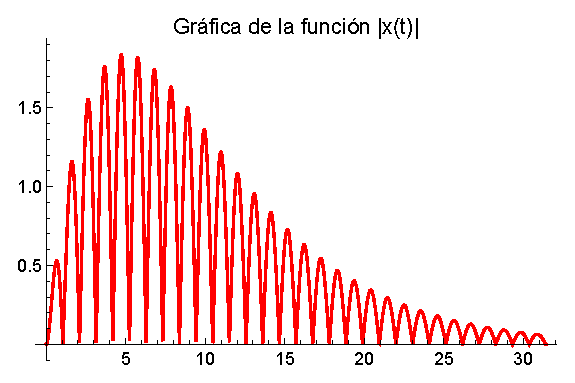
\includegraphics[scale=1]{Imagenes/Ejemplo_Resonancia_02.eps}
%     \caption{Gráfica del valor absoluto de la solución $x(t)$.}
% \end{figure}
% \end{frame}
% \begin{frame}[fragile]
% \frametitle{Gráfica con una envolvente}
% \begin{lstlisting}[language=Mathematica]
% Plot[{sol, curva}, {t, 0, 10 Pi}, PlotLabel -> "Grafica de la funcion x(t) y una envolvente", 
% LabelStyle -> Directive[FontSize -> 12], PlotStyle -> {Red, Blue}]
% \end{lstlisting}
% La siguiente figura es la que se obtiene:
% \end{frame}
% \begin{frame}
% \frametitle{Gráfica de $x(t)$ y una envolvente}
% \begin{figure}[H]
%     \centering
%     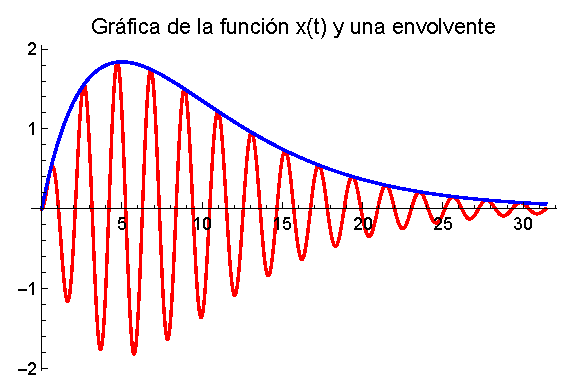
\includegraphics[scale=1]{Imagenes/Ejemplo_Resonancia_03.eps}
%     \caption{Solución obtenida con \texttt{Mathematica} y una curva envolvente.}
% \end{figure}
% \end{frame}
% \begin{frame}[fragile]
% \frametitle{Gráfica con las dos envolventes}
% \begin{lstlisting}[language=Mathematica]
% Plot[{sol,curva, -curva},{t,0,10 Pi},PlotStyle->{{Red,Dashing[None]},{Blue,Dashing[None]}, {Blue,Dashing[None]}}]
% \end{lstlisting}
% La dos curvas envolventes se muestran en la siguiente figura:
% \end{frame}
% \begin{frame}
% \frametitle{Gráfica de $x(t)$ y las curvas envolventes}
% \begin{figure}[H]
%     \centering
%     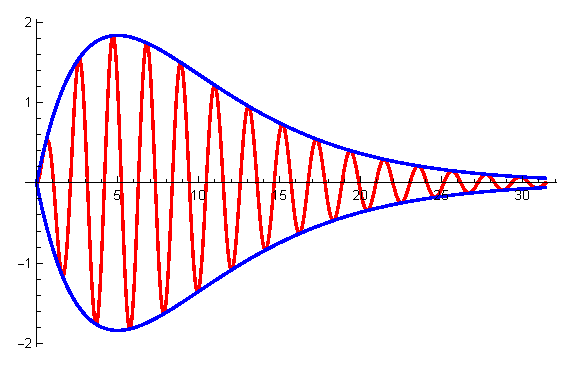
\includegraphics[scale=1]{Imagenes/Ejemplo_Resonancia_04.eps}
%     \caption{Solución obtenida con \texttt{Mathematica} y las curvas envolventes.}
% \end{figure}
% \end{frame}
% \begin{frame}
% \frametitle{Gráfica con otros elementos}
% Usando las herramientas de dibujo se puede agregar otros elementos como texto normal o texto con formato matemático, como en la siguiente figura.
% \\
% \bigskip
% \pause
% Agregar estos elementos favorecen una mejor lectura para la gráfica que se esté generando.
% \end{frame}
% \begin{frame}
% \frametitle{Gráfica de $x(t)$ y las curvas envolventes}
% \begin{figure}[H]
%     \centering
%     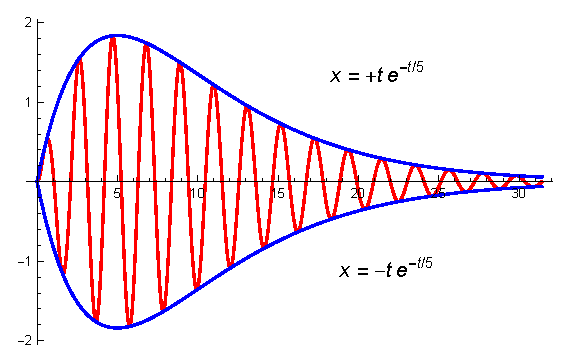
\includegraphics[scale=1]{Imagenes/Ejemplo_Resonancia_05.eps}
%     \caption{Solución obtenida con \texttt{Mathematica}, las curvas envolventes y texto agregado en la gráfico.}
% \end{figure}
% \end{frame}
% \subsection{Masas acopladas}
% \begin{frame}
% \frametitle{Resolviendo el ejercicio}
% Ahora trabajaremos el mismo ejercicio del sistema de masas acopladas con dos resortes, se mostrará el código utilizado en \texttt{Mathematica}.
% \end{frame}
% \begin{frame}[fragile]
% \frametitle{Código en \texttt{Mathematica}}
% \begin{lstlisting}[language=Mathematica]
% Clear[x, y, t] |\pause|
% sys = {x''[t] == -10 x[t] + 4 y[t], y''[t] == -4 y[t] + 4 x[t]} |\pause|
% paso1 = LaplaceTransform[sys, t, s] |\pause|
% paso2 = paso1 /. {x[0] -> 0, x'[0] -> 1, y[0] -> 0, y'[0] -> -1} |\pause|
% paso3 = Solve[paso2, {LaplaceTransform[x[t], t, s], LaplaceTransform[y[t], t, s]}] // Simplify
% \end{lstlisting}    
% \end{frame}
% \begin{frame}[fragile]
% \frametitle{Código en \texttt{Mathematica}}
% \begin{lstlisting}[language=Mathematica]
% x[t_]=InverseLaplaceTransform[paso3[[1,1,2]],s,t] |\pause|
% y[t_] = InverseLaplaceTransform[paso3[[1, 2, 2]], s, t] |\pause|
% Plot[{x[t],y[t]},{t,0,4Pi}, PlotLegends->{"Subscript[x, 1](t)", "Subscript[x, 2](t)"}, PlotLabel->"Grafica del movimiento de las masas acopladas", LabelStyle->Directive[FontSize->12]]
% \end{lstlisting}    
% \end{frame}
% \begin{frame}
% \frametitle{Gráfica de $x_{1}(t)$ y $x_{2}(t)$}
% \begin{figure}[H]
%     \centering
%     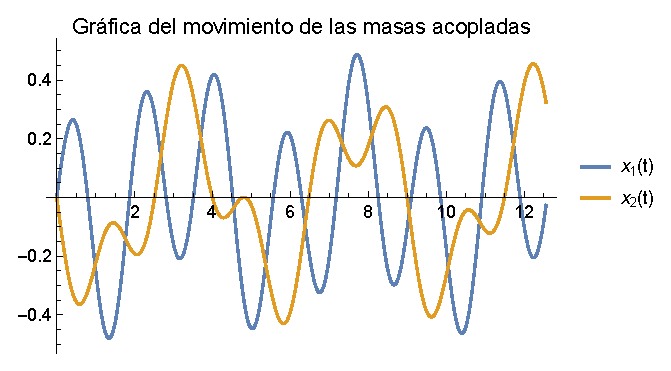
\includegraphics[scale=0.95]{Imagenes/Ejercicio_masas_acopladas_01.eps}
%     \caption{Gráfica obtenida usando las funciones de la transformada de Laplace y la transformada inversa para el sistema de dos masas acopladas mediante resortes.}
% \end{figure}
% \end{frame}
\begin{frame}   
\frametitle{Extendiendo la interpretación}
Ahora contamos con más elementos que aportarán a la interpretación del resultado: si graficamos $x_{1}$ vs $x_{2}$ obtendremos el \texttt{espacio fase} del sistema.
\end{frame}
% \begin{frame}[fragile]
% \frametitle{Código en \texttt{Mathematica}}
% \begin{lstlisting}[language=Mathematica]
% ParametricPlot[{x[t], y[t]}, {t, 0, 4 Pi}, AspectRatio -> 1, PlotLabel -> "Espacio fase de las masas acopladas", LabelStyle -> Directive[FontSize -> 12]]
% \end{lstlisting}    
% \end{frame}
\begin{frame}
\frametitle{Espacio fase del sistema}
\begin{figure}[H]
    \centering
    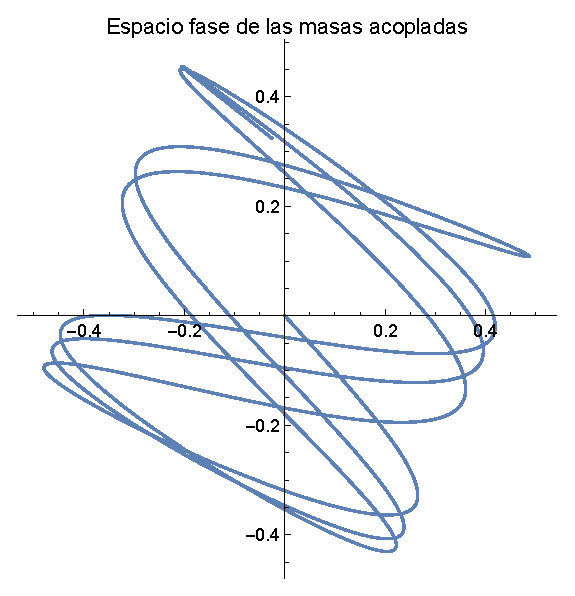
\includegraphics[scale=0.7]{Imagenes/Ejercicio_masas_acopladas_03.eps}
\end{figure}
\end{frame}
\end{document}